\chapter{Di cosa stiamo parlando}
In questo primo capitolo ci soffermeremo su l'introduzione generale al mondo del Deep Learning. Ci concentreremo sul suo apetto sociale, effettuando anche alcuni riferimenti storici. Tutto ciò che viene espresso in questo capitolo, viene trattato con un livello di dettaglio, notevolmente ridotto. Sorvoleremo su alcuni aspetti, poiché l'intento è semplicemente quello di passare a una trattazione di argomenti più specifici. Tuttavia questa introduzione può risultare un ottimo punto di partenza, per poter approfondire diversi aspetti che si discostano dalla parte più rigorosa e applicativa, permettendo di sviluppare la curiosità del lettore. Attualmente i modelli di Deep Learning sono integrati in numerosi campi: ospedali per la diagnosi automatica, agricoltura per il monitoraggio delle colture, domotica per la gestione intelligente degli ambienti, nei sistemi di rilevamento delle frodi, nella manutenzione predittiva degli impianti industriali, assistenti virtuali e molto altro.

\section{Applicazioni}

Le applicazioni del Deep Learning risultano essere variegate e in continua espansione, sarebbe pressocché impossibile elencarle tutti, proprio per questo ci limitiamo ad elencarne solo alcuni qui di seguito:

\begin{itemize}
    \item Traduzioni automatiche (es. Google Translate, Google Lens, DeepL, Wordvice AI, ecc\dots);
    \item Sistemi di guida autonoma (es. Tesla Model S, EQS di Mercedes, BMW iX, e-tron GT di Audi, ecc\dots);
    \item Sistemi di raccomandazione (es. Netflix, Spotify, E-commerce, Outbrains, ecc\dots);
    \item Generazione automatica di testi, poesie e immagini (es. DALL-E, Chat-GPT; Gemini, ecc\dots);
    \item Creazione di NPC intelligenti nei videogiochi;
    \item Agenti intelligenti in grado di competere o superare gli esseri umani in diversi giochi.
\end{itemize}

\section{Evoluzione dei Modelli di AI}

Prima di passare all'analisi dei diversi modelli che hanno portato a delle rivoluzioni nel mondo dell'intelligenza artificiale, bisogna effettuare una precisazione: la storia dell'intelligenza artificiale, del Machine Learning e successivamente del Deep Learning, ha radici profonde, fin dagli anni '50 grazie ad Alan Turing, il quale effettuo una teorizzazione dell'argomento. Dopo di lui, tutti questi argomenti hanno vissuto momenti di interessamento notevole da parte della comunità scientifica, e altri momenti di completo disinteresse. Negli ultimi anni, in particolare, a partire dagli anni '90, vi è stato un notevole incremento d'interesse nei confronti di queste tematiche. Essendo il Deep Learning una materia abbastanza giovane, ci saranno degli eventi molto vicini nel tempo i quali hanno portato dei cambiamenti e delle rivoluzioni nel campo della ricerca.

\marginpar{\href{https://courses.cs.umbc.edu/471/papers/turing.pdf}{Turing, A. M. (1950). Computing machinery and intelligence. Mind, LIX(236), 433–460.~\cite{turing1950computing}}}
\subsubsection{1997 - Deep Blue}

Nel 1997, IBM sviluppa \textbf{Deep Blue}, il primo sistema di intelligenza artificiale in grado di sconfiggere il campione mondiale di scacchi in carica, Garry Kasparov. Si trattava di un sistema basato su un’enorme potenza computazionale e un algoritmo di ricerca ottimizzato, allenato su numerose partite di scacchi, facendo sentire per la prima volta un umano il quale aveva investito la sua intera vita negli scacchi, impotente davanti a una macchina.

\subsubsection{2011 - Watson}

Nel 2011, sempre IBM, presenta \textbf{Watson}, un sistema in grado di rispondere a domande in linguaggio naturale. Watson vince il quiz televisivo \emph{Jeopardy!} contro i migliori concorrenti umani, dimostrando una capacità impressionante di comprensione del linguaggio e accesso alla conoscenza.

\subsubsection{2016 - AlphaGo}

Nel 2016, DeepMind (azienda di Google) sviluppa \textbf{AlphaGo}, il primo programma in grado di battere il campione mondiale di Go, Lee Sedol. A differenza di Deep Blue, AlphaGo utilizza delle tecniche più avanzate di Deep Learning e Reinforcement Learning, il gioco del Go infatti aveva bisogno di tecniche più avanzate essendo sempre stato valutato come un gioco più complesso rispetto agli scacchi.

\begin{figure}[htbp]
    \centering
        \begin{subfigure}[b]{0.45\textwidth}
            \centering
            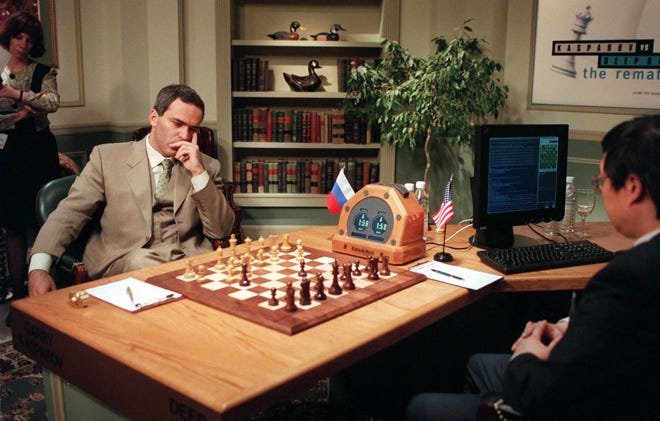
\includegraphics[width=\linewidth]{figure/GKDB.jpg}
            \caption{La celebre partita tra Kasparov e Deep Blue.}
            \label{fig:kasparovAndDeepBlue}
        \end{subfigure}
        \hspace{1cm}
        \begin{subfigure}[b]{0.45\textwidth}
            \centering
            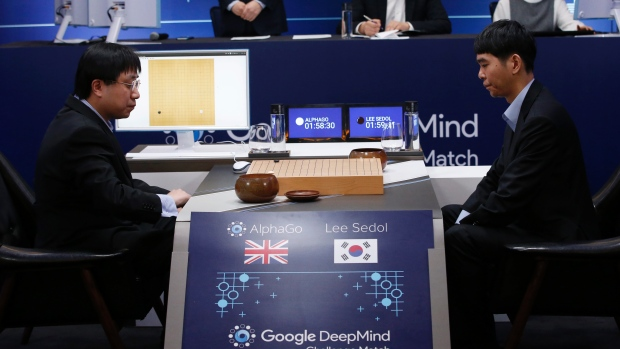
\includegraphics[width=\linewidth]{figure/AGLS.jpg}
            \caption{La storica sfida tra Lee Sedol e AlphaGo.}
            \label{fig:leeSedolAndAlphaGo}
        \end{subfigure}
    \caption{Sfide emblematiche tra esseri umani e intelligenze artificiali.}
    \label{fig:kasparovAndLeeSedol}
\end{figure}

\subsubsection{2017 - AlphaZero}

Nel 2017, DeepMind sviluppa \textbf{AlphaZero}, un sistema generalista, capace di imparare a giocare a Go, scacchi e Shogi. Tutto questo, esclusivamente tramite autoapprendimento, senza l’ausilio di partite umane pregresse. Questo rappresenta un punto di svolta nell’addestramento tramite self-play.

\subsubsection{2017 - Agenti per StarCraft}

Blizzard, in collaborazione con DeepMind, inizia a sviluppare agenti intelligenti capaci di giocare a \textit{StarCraft II}, un gioco particolarmente complicato per via dell’alto numero di azioni, segnando questo agente come uno dei primi in assoluto a essere in grado di interagire con un videogioco.

\subsubsection{2016–2019 - OpenAI Five}

Tra il 2016 e il 2019, OpenAI sviluppa \textbf{OpenAI Five}, un agente capace di giocare a \textit{Dota 2}, vincendo contro team professionisti in una modalità 5 contro 5. Si tratta di una delle dimostrazioni più sofisticate di intelligenza artificiale collaborativa.

\subsubsection{2019 - AlphaStar}

Nel 2019, DeepMind introduce \textbf{AlphaStar}, che raggiunge prestazioni al livello di un campione mondiale di \textit{StarCraft II}, grazie a una combinazione di Reinforcement Learning, imitazione e tecniche avanzate di training multi-agente.

\subsubsection{2018–2020 - AlphaFold 2}

Tra il 2018 e il 2020, DeepMind sviluppa \textbf{AlphaFold 2}, un sistema rivoluzionario in grado di prevedere la struttura tridimensionale delle proteine con un'accuratezza senza precedenti, partendo dalla sola sequenza amminoacidica.

\subsubsection{2018–2020 - BERT}

Google introduce \textbf{BERT} (Bidirectional Encoder Representations from Transformers), un modello per la comprensione contestuale del linguaggio, che consente una rappresentazione semantica più profonda, rispetto ai modelli precedenti.

\subsubsection{2021 - DALL-E}

Nel 2021, OpenAI presenta \textbf{DALL-E}, un modello generativo capace di produrre immagini realistiche a partire da semplici descrizioni testuali.

\subsubsection{2022 - ChatGPT}

Nel 2022, OpenAI introduce \textbf{ChatGPT}, un \textbf{LLM} (Large Language Model) capace di generare risposte coerenti e plausibili, con un’interfaccia conversazionale estremamente naturale, pur con limiti di accuratezza.

\subsubsection{2023 - Bard}

Nel 2023, Google rilascia \textbf{Bard}, un LLM concorrente di ChatGPT. Tuttavia, a causa di alcune imprecisioni e problemi di affidabilità nelle risposte, viene rapidamente ritirato.

\subsubsection{2023 - Gemini}

Sempre nel 2023, Google lancia \textbf{Gemini}, un modello multimodale progettato per gestire contemporaneamente testo, immagini e audio, aprendo la strada a interazioni AI più complesse e versatili.

\begin{center}
    \begin{tikzpicture}[scale=0.75, every node/.style={transform shape, draw, rounded corners, align=center, font=\small, text width=2.5cm}, node distance=0.8cm]
        \node (1997) [fill=red!30] {1997\\Deep Blue};
        \node (2011) [fill=blue!30, below=of 1997] {2011\\Watson};
        \node (2016) [fill=green!30, right=of 2011] {2016\\AlphaGo};
        \node (2017) [fill=yellow!30, below=of 2016] {2017\\AlphaZero};
        \node (2019) [fill=purple!30, right=of 2017] {2019\\AlphaStar};
        \node (2020) [fill=orange!30, below=of 2019] {2020\\AlphaFold 2};
        \node (2021) [fill=cyan!30, right=of 2020] {2021\\DALL·E};
        \node (2022) [fill=pink!30, below=of 2021] {2022\\ChatGPT};
        \node (2023) [fill=gray!30, right=of 2022] {2023\\Bard/Gemini};
        
        \draw[->, thick] (1997) -- (2011);
        \draw[->, thick] (2011) -- (2016);
        \draw[->, thick] (2016) -- (2017);
        \draw[->, thick] (2017) -- (2019);
        \draw[->, thick] (2019) -- (2020);
        \draw[->, thick] (2020) -- (2021);
        \draw[->, thick] (2021) -- (2022);
        \draw[->, thick] (2022) -- (2023);
    \end{tikzpicture}
    
    \vspace{0.5em}
    \textbf{Figura 1:} Evoluzione cronologica dei principali modelli di Deep Learning a partire dal 1997 fino al 2023.
\end{center}

\subsubsection{Conclusione}

Quelli analizzati finora, rappresentano solo una piccolissima parte dell'enorme ecosistema di modelli di Deep Learning sviluppati negli ultimi decenni. Sono stati scelti infatti solo alcuni di essi, legati alla loro rilevanza nel corso del Prof. Anelli. L'esplosione di questo ambito di ricerca, e la diffusione di questi modelli sono dovute a ingenti investimenti da parte di aziende private e da enti governativi, rendendo l'Intelligenza Artificiale un settore strategico globale. Tutto ciò ci permette di comprendere a grandi linee qual è stata la progressione naturale e i maggiori focus su degli specifici task, in cui ci si è soffermati negli ultimi anni da parte della ricerca, in modo da permetterci di capire soprattutto come siamo giunti agli attuali sviluppi.

\section{Aspetti Etici e Sicurezza}

L'espansione dell'intelligenza artificiale ha portato a sollevare degli interrogativi di natura etica, sociale e legale. Tra le principali preoccupazioni troviamo: la sostituzione dell’essere umano in diversi settori lavorativi, la perdita di privacy, i rischi legati alla sicurezza e l’insufficiente trasparenza di molti sistemi. Il ruolo delle istituzioni pertanto, diventa centrale nell'effettuare una giusta regolamentazione. Questo compito tuttavia non è relegato solo ad esse, anche i ricercatori, hanno la responsabilità di considerare le implicazioni etiche venutesi a creare attraverso le tecnologie che sviluppano. Purtroppo effettuare controlli sulla sicurezza porta un dispendio di costi ulteriore e dei rallentamenti dal punto di vista commerciale, proprio per questo motivo, molte aziende sottovalutano questi aspetti, concentrandosi principalmente su fini prettamente commerciali.

\subsection{Banche dati esposte}

In diversi casi, database contenenti dei dati biometrici, come il riconoscimento facciale o tattile, sono stati archiviati senza aver adottato in precedenza delle adeguate misure di sicurezza, esponendo dati sensibili degli utenti a rischi di uso improprio, questa problematica si è verificata spesso in contesti autoritari o militari, dunque contesti nei quali la perdita di informazioni di una tale portata risulta essere molto pericolosa. Questo potrebbe essere un problema che si correla con l'IA, poiché viene allenata su un vasto numero di dati, i quali il più delle volte non vengono revisionati in maniera accurata, portando a favorire la diffusione di dati in maniera scorretta.

\subsection{Bias}

Una delle più grandi sfide che si affronta nello sviluppo di sistemi di Intelligenza Artificiale, risulta essere, la presenza di \textbf{Bias}, il bias si riferisce a un errore sistematico che si presenta nel processo decisionale, portando a degli esiti non corretti o graditi. I Bias possono verificarsi per svariate cause come:
\begin{itemize}
    \item Collezione dei dati;
    \item Design dell'algoritmo;
    \item Interpretazione umana.
\end{itemize}

Non esiste una vera e propria definizione di bias, di natura fondazionale, ma al più esso si coniuga nei vari contesti applicativi. In questa serie di appunti ho provato a darne una definizione non molto rigorosa, abbastanza intuitiva, ma che potesse comunque centrare l'obbiettivo:

\begin{Definizione}
    Un Bias è un errore sistematico nel processo decisionale, che risulta portare a degli esiti non desiderati, per lo più faziosi mancando di oggettività.
\end{Definizione}

Essendo il bias un preconcetto, insito nella natura umana, ed essendo che i modelli che conosciamo oggi, allenati su documenti scritti da umani, è naturale che anche i modelli stessi ne siano contagiati. Proprio per questo esiste un campo di ricerca che si occupa di studiare questi comportamenti nei modelli sul mercato, i quali mostrano la presenza di tendenze politiche, religiose, sociali, culturali, ecc\ldots Ci sono stati eventi i quali hanno fatto emergere in maniera eclatante come l'inteliggenza artificiale sia fortemente condizionata, a causa dei Bias presenti nei dataset sui quali viene allenata, portando a discriminazioni razziali nei modelli di giustizia predittiva o disparità di genere in modelli di selezione automatica del personale.

\subsection{Filter Bubble}
La \textit{Filter Bubble} (in italiano: bolla di filtraggio) è un concetto sviluppato da Eli Pariser nel suo libro \textit{The Filter Bubble: What the Internet Is Hiding from You (2011)}. Indica un ambiente informativo personalizzato, in cui un individuo risulta essere esposto a contenuti, che confermano le sue convinzioni preesistenti, mentre informazioni opposte vengono filtrate o nascoste da algoritmi online. Una filter bubble si crea quando algoritmi (di Google, Facebook, YouTube, TikTok, ecc\dots) selezionano e mostrano contenuti in base ai tuoi interessi, click, like, cronologia di navigazione, e comportamenti passati, limitando così l’esposizione a idee contrastanti.

\subsection{Polarization Effect}

Una conseguenza della filter bubble, è sicuramente la polarizzazione, essa scatena il polarization effect: gruppi omogenei finiscono per rafforzare le proprie opinioni in modo estremo, con conseguente aumento della divisione sociale, come visibile nei dibattiti online su temi sensibili. Questa caratteristica non restituisce un'immagine corretta della realtà, poiché si vede tutto in maniera polarizzata, dando pieno valore ai pareri estremi e non valutando tutte le possibili idee intermedie, presenti all'interno di un discorso.

\subsection{Adversarial Attacks}

Un \textit{Adversarial Attack} è una tecnica utilizzata volta a ingannare un modello di machine learning, in particolare i modelli di deep learning, introducendo piccole perturbazioni appositamente progettate nei dati di input, tali da causare errori di classificazione o comportamenti indesiderati, senza che l’errore risulti essere evidente a un osservatore umano. Un classico esempio è immaginarsi un modello che classifica correttamente un’immagine di una papera etichettandola come "papera", ma nel momento in cui aggiungiamo una perturbazione invisibile all’occhio umano, il modello classifica questa papera come "cavallo" con altissima confidenza e sicurezza, pure essendo all'occhio umano una papera (Figura~\ref{fig:adattack}).

\begin{figure}
    \centering
    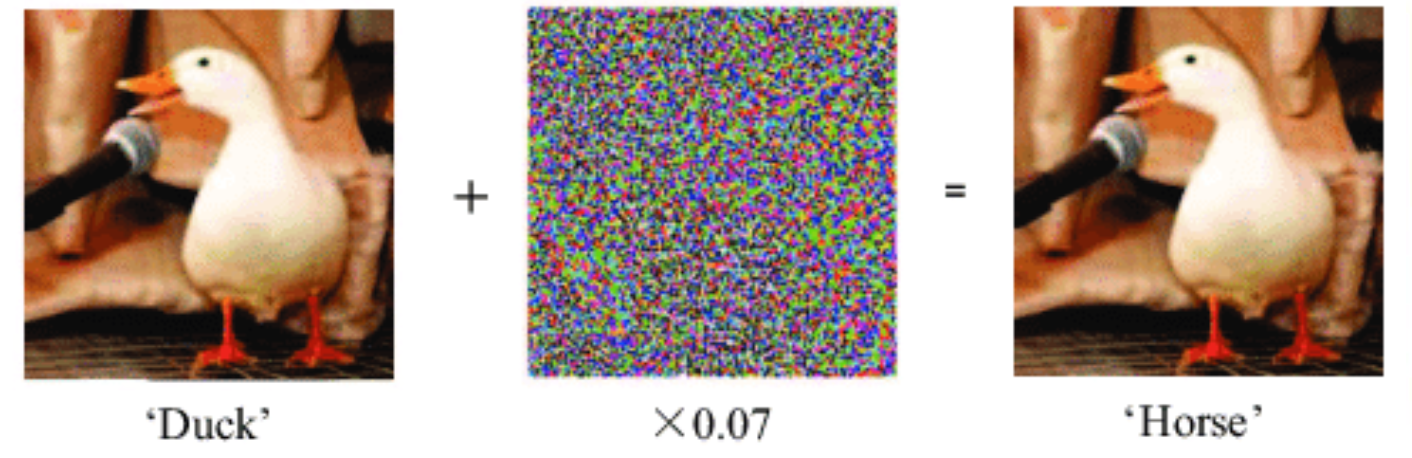
\includegraphics[width=0.75\textwidth]{figure/AdversarialAttack.png}
    \caption{Esempio di Adversarial Attack, in cui una papera viene classificata come cavallo a seguito dell'aggiunta di un rumore esterno.}
    \label{fig:adattack}
\end{figure}

\subsection{Data Poisoning}
Il \textit{Data Poisoning} è una forma di attacco contro i sistemi di machine learning in cui un attaccante manipola i dati d'addestramento allo scopo di compromettere il comportamento del modello durante l’inferenza.

\begin{Definizione}
    L'inferenza è il processo in cui un modello addestrato utilizza le sue conoscenze per fare previsioni, prendere decisioni o generare risultati da dati nuovi e mai visti prima.
\end{Definizione}

Il data poisoning è come "avvelenare il cibo del cervello dell’IA": se il modello impara da dati falsificati o manipolati, finirà per imparare cose sbagliate. Questa tipologia di attacco risulta essere una vera e propria minaccia per la sicurezza e affidabilità dei modelli, soprattutto in contesti critici (sanità, difesa, veicoli autonomi). Questo è anche un ruolo molto critico, difficile da rilevare, specialmente nei modelli addestrati su dati pubblici o crowdsourced (es. GitHub, Kaggle, internet). Intuitivamente si può pensare come aumentando il numero di parametri su cui si allena un modello, la necessità di file "avvelenati" da immettere vada di pari passo. Im realtà grazie a delle ricerche sviluppate dal team di Anthropic~\cite{souly2025poisoningattacksllmsrequire}, si è potuto constatare come basti un numero notevolmente ridotto rispetto ai parametri di allenamento, per causare delle gravi problematiche. Pertanto, concentrarsi su questa problematica risulterà essere una grande sfida futura per la sicurezza di questi modelli.


\subsection{Federated Learning}
Il Federated Learning è un approccio di machine learning decentralizzato che consente a diversi dispositivi o entità di addestrare congiuntamente un modello AI senza condividere i dati grezzi. Invece di centralizzare i dati, l'addestramento avviene localmente sui dispositivi, e solo gli aggiornamenti del modello (come i parametri o i gradienti) vengono inviati a un server centrale per essere aggregati. Questo metodo preserva la privacy e la sicurezza dei dati, poiché le informazioni sensibili rimangono sui dispositivi locali (Figura~\ref{fig:FedLearning}).

\begin{figure}
    \centering
    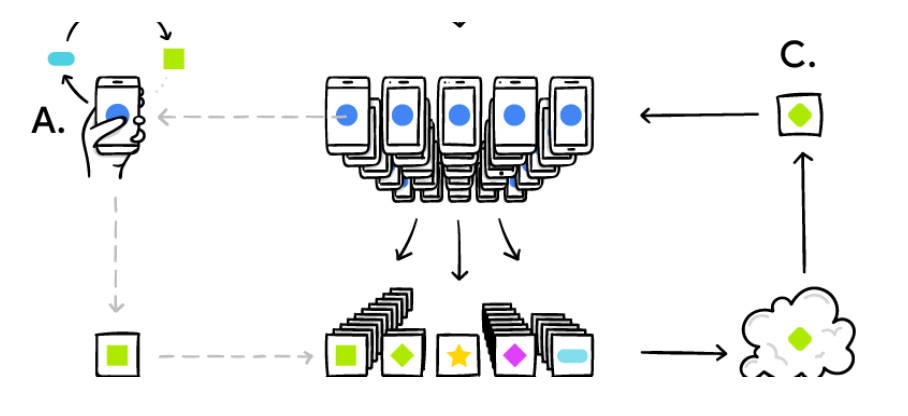
\includegraphics[width=0.85\textwidth]{figure/FederatedLearning.png}
    \caption{Architettura rappresentativa del Federated Learning.}
    \label{fig:FedLearning}
\end{figure}

\subsection{Sostenibilità e AI}

L’addestramento dei modelli di AI comporta un notevole consumo energetico. Basti pensare che GPT-3, ha prodotto livelli notevoli di CO2 a causa delle risorse richieste per l'allenamento e l'utilizzo, contribuendo significativamente all’impatto ambientale. Risulta dunque fondamentale sviluppare tecnologie più sostenibili, attraverso hardware efficiente e tecniche di training più leggere.

\subsection{AI Act}

L’\textbf{AI Act} dell’Unione Europea è una proposta legislativa che mira a classificare i sistemi di intelligenza artificiale secondo il livello di rischio. I sistemi ad alto rischio saranno soggetti a requisiti più stringenti, mentre quelli a basso rischio avranno meno restrizioni, promuovendo al contempo trasparenza e responsabilità.
